%%% LaTeX Template: Article/Thesis/etc. with colored headings and special fonts
%%%
%%% Source: http://www.howtotex.com/
% vim: set spell spelllang=es syntax=tex :

\documentclass[12pt]{article}
\usepackage{styles/apuntes-estilo}
\usepackage{fancyhdr,lastpage}
\usepackage{hyperref}
\usepackage[inline]{enumitem}
\usepackage{xurl}

\def\maketitle{

\makeatletter{
    \color{blue} \centering \huge \sc
    \textbf{
        Trabajo práctico de laboratorio N° 10\\
        \large \vspace*{-8pt} \color{black}
        Introducción al shell del sistema GNU/LINUX
        \vspace*{8pt}
    }\\
    \small Fecha de finalización: 10 de Junio
    \par
}

\makeatother

\makeatletter
% vim: set spell spelllang=es syntax=tex :
 {\centering \small 
    Introducción a la computación\\
    Departamento de Ingeniería de Computadoras \\
    Facultad de Informática - Universidad Nacional del Comahue \\
    \vspace{20pt} }
\makeatother

\vspace{-2.5cm}
\mbox{\hspace{-1cm}\includegraphics[width=3cm,height=3cm]{logos/uncoma.pdf}\hspace{13cm}
    \includegraphics[width=2.9cm,height=2.9cm]{logos/fai.pdf}}



}

% Custom headers and footers
\fancyhf{} % clear all header and footer fields
\fancypagestyle{plain}{\fancyhf{}}
\pagestyle{fancy}
\lhead{\footnotesize Laboratorio N° 1 - Introducción al shell del sistema GNU/LINUX}
\rhead{\footnotesize \thepage\ }

\def\ti#1#2{\texttt{#1} & #2 \\ }

\newcommand{\bash}{\textbf{\emph{BASH}}}

\begin{document}

\thispagestyle{empty}
\maketitle
\setlength{\parindent}{1pt}

\textbf{Lectura obligatoria:}

\vspace{-2\topsep}
\begin{itemize}

    \itemsep2pt \parskip0pt \parsep0pt

    \item Apunte del shell de Linux:
        \url{http://pedco.uncoma.edu.ar/mod/resource/view.php?id=207175}

    \item Apunte introductorio a \bash:
        \url{http://pedco.uncoma.edu.ar/mod/resource/view.php?id=244968}

    \item Linux Man Pages Online: \url{https://linux.die.net/man/}

\end{itemize}

A continuación, se realizarán una serie de ejercicios para los cuales
necesitará acceso a una computadora con el sistema operativo Linux (o una
Máquina Virtual corriendo Linux) y las siguientes aplicaciones:

\vspace{-2\topsep}
\begin{itemize}

    \itemsep2pt \parskip0pt \parsep0pt

    \item   Intérprete de comandos \bash y demás utilidades que se encuentran
        en la mayoría de las distribuciones de Linux.

    \item   Un editor de texto en la interfaz de línea de comando o gráfica.

\end{itemize}

NOTA: para un tutorial de conexión remota desde Windows a su usuario de alumno
FI (creado por la Facultad de Informática oportunamente), dirijase a
\ref{subsec:anexoI} Anexo I: Conexión desde entorno Windows a usuario de
alumno FI\\

NOTA 2: para un tutorial de conexión remota desde Linux a su usuario de alumno
FI (creado por la Facultad de Informática oportunamente), dirijase a
\ref{subsec:anexoII} Anexo II: Conexión desde entorno Linux a usuario de
alumno FI\\

El sistema operativo controla diferentes procesos de una computadora. Uno de
ellos es el intérprete de comandos o \emph{shell}. Este es un programa que
permite al usuario interactuar con el Sistema Operativo. Permite iniciar
(ejecutar) otros programas así como también tiene comandos propios que no
necesitan de otros programas, como por ejemplo comandos para movernos en la
estructura de directorios. En este práctico, utilizaremos el intérprete
\emph{BASH (Bourne-Again SHell)}, muy popular en el mundo de Linux.

Dicho programa debe ser ejecutado en lo que llamamos Terminal o Consola, que
es otro programa que nos permite interactuar mediante el teclado (ingresar
caracteres) y ver los resultados de la ejecución de otros programas en la
pantalla. Al iniciar una consola o terminal de textos, automáticamente se
inicia el \emph{shell} \bash, que es con el que el usuario realmente
interactúa (más abajo se explica esto con un ejemplo).

\section{Sistemas de archivos}

El concepto de directorios (comúnmente llamados ``carpetas'') y archivos es
hoy en día familiar a los usuarios de computadoras, en general el usuario se
maneja visualmente con el ratón y el Explorador de Archivos, utilizando estos
para acceder a los directorios, abrir archivos, ejecutar programas, etc.
Podemos pensar el sistema de archivos como una forma de organizar todo el
contenido en el dispositivo de almacenamiento. Los archivos son datos
concretos, utilizan espacio físico del dispositivo, mientras que los
directorios sirven para organizar ``lógicamente'' las cosas, igual que una
persona tiene estanterías y cajones en un escritorio para organizar sus
papeles.

La figura \ref{arbolDirectorios} muestra un esquema de como se puede pensar en
una estructura de directorios y archivos. \textbf{A}, \textbf{B}, \textbf{C},
\textbf{D}, \textbf{E}, \textbf{G} y \textbf{J} son directorios, \textbf{F},
\textbf{H}, \textbf{I}, \textbf{K}, \textbf{L}, \textbf{M}, \textbf{N} y
\textbf{O} son archivos.

\begin{figure}[!htb]

    \centering

    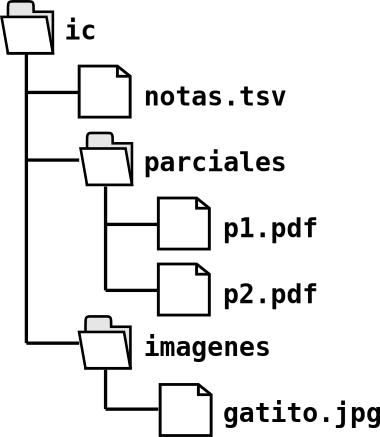
\includegraphics[height=0.45\textheight]{img/directorios.pdf}

    \caption{Árbol de directorios.}

    \label{arbolDirectorios}

\end{figure}

Cuando se inicia el intérprete de comandos, éste se posiciona en una
determinada carpeta, es decir, los comandos que se escriben afectarán
directamente al contenido de dicha carpeta.

En general, al iniciar una consola de texto, junto con un intérprete de
comandos, se posiciona al usuario en la carpeta personal o \textbf{``HOME''}
(en Linux en general es \emph{``/home/usuarioX''}). Desde aquí el usuario
puede navegar por sus archivos y ejecutar comandos.

Además, existen dos formas de hacer referencia a los directorios y a los
archivos en el intérprete, absoluta y relativa. Cuando utilizamos la forma
absoluta se escribe todo el camino desde la carpeta inicial (en \emph{Linux}
se denota con el símbolo \emph{``/''}) hasta la ubicación deseada. Ejemplos de
uso absoluto: \emph{/home/usuario/trabajo1}, \emph{/etc}, \emph{/tmp}, etc.

El modo relativo sirve para hacer referencia a un directorio que se encuentra
``cerca'' del directorio de trabajo actual en la jerarquía, como por ejemplo
el directorio directamente superior o inferior.

Por ejemplo, las siguientes son direcciones relativas:

\vspace{-2\topsep}
\begin{itemize}

    \itemsep2pt \parskip0pt \parsep0pt

    \item \emph{../} (directorio inmediatamente superior)

    \item \emph{./trabajo1} (directorio trabajo1 ubicado dentro del directorio
        actual)

    \item \emph{../../archivoX} (archivo ubicado dos directorios más arriba en
        la jerarquía)

\end{itemize}

\subsection{Entrando en calor con el \emph{shell} \bash}

\begin{enumerate}

    \item Inicie el programa mate terminal: \textbf{Aplicaciones →
        Herramientas del sistema → Terminal de mate}.

        Una vez iniciado, el \emph{shell} \bash en la terminal espera que se
        escriban órdenes para ejecutar (comandos). Ejecute y analice
        cuidadosamente la siguiente secuencia de comandos en el intérprete
        \bash (luego de los comandos y parámetros debe presionar
        \emph{ENTER}).

        Puede consultar el manual de cada uno de los comandos utilizados,
        usando el comando \emph{``man nombre\_del\_comando''}, donde se
        muestran opciones de uso y se explica la funcionalidad del mismo.

\begin{center}

    \begin{tabular}[t]{l l }
    \hline
        \textbf{Comandos y parámetros} & \textbf{Descripción} \\
    \hline
    \hline
        mkdir e &  \#crear un directorio de nombre ``e'' \\
        cd e &  \#cambiar el directorio actual a ``e'' \\
        mkdir h1 &  \#crear un directorio ``h1'' \\
        mkdir h2 &  \#crear un directorio ``h2'' \\
        cd h1 &  \#cambiar el directorio actual a ``h1'' \\
        nano a.txt &  \#crear un archivo de texto y guardarlo \\
        pwd &  \#imprime el directorio actual \\
        cd .. &  \#cambiar el directorio actual al directorio padre \\
        pwd &  \#imprime el directorio actual \\
        cd .. &  \#cambiar el directorio actual al directorio padre \\
        pwd &  \#imprime el directorio actual \\
        ls &  \#listado del directorio actual \\
        ls -R &  \#listado recursivo de los contenidos \\
        mv e/h1/a.txt e/h2/a.txt &  \#mueve el archivo a.txt a otro directorio \\
        rm e/h2/ab.txt &  \#eliminar el archivo ab.txt, falla por que no
        existe\\
        rm e/h2/a.txt &  \#eliminar el archivo a.txt \\
        rmdir e/h1 &  \#elimina el directorio h1 \\
    \hline
    \end{tabular}

\end{center}

    \item Realice un esquema visual como el de la figura
        \ref{arbolDirectorios}, que muestre la estructura de directorios
        resultante de ejecutar la siguiente secuencia de comandos:

        \begin{verbatim}
mkdir e
cd e
mkdir h1
mkdir h2
cd h1
nano README
cd ..
cd h2
mkdir h2 h3
cd h2
nano otroArchivo
cd ../../
nano a3.txt
        \end{verbatim}

    \item Utilizando los comandos vistos en el listado, reproduzca la
        estructura de directorios y archivos de la figura
        \ref{arbolDirectorios}, respetando mayúsculas y nombres de los
        archivos. Esta estructura será utilizada en los subsiguientes incisos.

    \item Utilizando la jerarquía de directorios generados en el inciso
        anterior, posicione el intérprete en el directorio ``A'', y realice
        las siguientes acciones:

    \begin{enumerate}

        \item Elimine el archivo ``M'' sin cambiar de directorio.

        \item Mueva los archivos ``H'' e ``I'' a la carpeta ``G''.

        \item Elimine la carpeta ``D''.

        \item Posicione el intérprete en el directorio ``G''.

        \item Sin cambiar de directorio, listar el contenido del directorio
            ``J'' usando directorios relativos.

        \item Sin cambiar de directorio, listar el contenido del directorio
            ``J'' usando directorios absolutos. Para armar una dirección
            absoluta puede usar el comando ``pwd'' para conocer como se
            conforma el camino completo hasta la ubicación actual.

    \end{enumerate}

    \item Explique las ventajas del uso de direcciones ``relativas'' a la
            hora de hacer referencia a otros archivos cercanos en la jerarquía
            al directorio de trabajo actual. Utilice un ejemplo.

    \item Liste el contenido del directorio ``J'', con el comando ``ls -l
        \emph{camino\_a\_J}''.  Analice la información que se muestra por
        pantalla, fecha de creación de los archivos, propietario de los
        archivos y tamaño de los archivos. Modifique alguno de los archivos en
        el editor de texto y vuelva a analizar la salida del comando ``ls
        -l''.

    \item Con el comando ``ls -l'' encuentre un archivo dentro del directorio
        ``/etc'' cuyo tamaño sea mayor a 4KiB, y liste el contenido de dicho
        archivo utilizando los comandos ``cat'', ``more'' y ``less''.

    Teclas útiles:

    \begin{itemize}

        \itemsep2pt \parskip0pt \parsep0pt

        \item cat: no tiene.

        \item more: ``q'' para salir, ``barra espaciadora'' avanzar página.

        \item less: ``q'' para salir, ``barra espaciadora'' avanzar página, y
            ``j'', ''k'' para subir y bajar.

    \end{itemize}

    \item Retorne a su directorio \textbf{HOME}. Para esto ejecute:
        (\textbf{Atención}: el signo \emph{\$} a partir de ahora representa el
        \emph{prompt} del \emph{shell} \bash, no debe escribirlo al ingresar
        cada comando)

        \begin{verbatim}
$ cd           # este es el comando para retornar a su HOME
$ pwd          # pwd le indica cuál es su directorio de trabajo actual
        \end{verbatim}

\end{enumerate}

\subsection{Archivos: nombre, tamaño, tipo, contenido.}

\begin{enumerate}

    \item Asegúrese de que su directorio de trabajo actual es su directorio
        \textbf{HOME} (comando: \emph{pwd}).

    \item Crear un directorio llamado ``misc'' (sin las comillas).

    \item Ingresar al directorio ``misc'' y copiar dentro del mismo los
        siguientes archivos (utilice rutas absolutas con el comando \emph{cp}):

\begin{verbatim}
/etc/passwd
/usr/share/sounds/alsa/Noise.wav
/bin/zcat
/bin/cpio
/usr/share/doc/zenity/NEWS.gz
/usr/share/doc//sudo/README
\end{verbatim}

    \item Una vez copiados, liste los archivos en el directorio misc. Usted
        debería observar que existen seis archivos:

        \begin{verbatim}
$ pwd
$ ls -l
        \end{verbatim}

    \item El comando ``ls'' anterior le ha entregado información sobre los
        archivos.  Indique el tamaño de cada archivo (en bytes y en KiB).

    \item Observe de qué tipo son los seis archivos en el directorio
        \emph{misc}.  Utilice el comando ``file archivo''. Ejemplo:

        \begin{verbatim}
$ file passwd
        \end{verbatim}

    \item Ahora analizaremos el contenido de cada archivo. Para realizar esta
        tarea obtendremos los primeros 32 bytes de cada archivo. Utilizaremos
        el programa ``hexdump'' para visualizar en base 16 (hexadecimal) el
        valor de cada byte. Ejemplo:

        \begin{verbatim}
$ hexdump -C cpio | head -2
        \end{verbatim}

        El comando anterior le presenta en pantalla el contenido de los
        primeros 32 bytes del archivo \emph{cpio}. Repita la operación para
        cada archivo en el directorio \emph{misc}. Registre los resultados.

    \item Escriba el contenido en base 2 (binario) de los primeros 4 bytes de
        cada archivo.

    \item Sabiendo que cada archivo en el sistema es almacenado en una memoria
        que únicamente puede mantener los datos utilizando componentes
        electrónicos biestables (que mantiene únicamente dos valores
        diferentes) analice y desarrolle un texto que intente explicar cómo es
        posible que los archivos en el sistema sean de diferente ``tipo'' si
        la computadora mantiene únicamente los datos en base 2.

\end{enumerate}

\clearpage
\subsection{Anexo I: Conexión desde entorno Windows a usuario de alumno FI}
\label{subsec:anexoI}

\begin{enumerate}

\item Ingresamos en el buscador de Windows y ponemos la palabra \emph{remoto}, lo que nos traerá como resultado la aplicación: “Conexión a Escritorio remoto”. Dicho procedimiento se ilustra en la Figura \ref{busquedaWindows}. 

\begin{figure}[!hb]

    \centering

    \includegraphics[width=0.5\textwidth]{img/tpLabImg1Win.pdf}

    \caption{Búsqueda de Escritorio Remoto Windows.}

    \label{busquedaWindows}

\end{figure}

\item Al hacer clic sobre el programa se nos abrirá la interfaz para ingresar
    la dirección a la cual queremos conectarnos según Figura \ref{escRemoto}.

    En donde dice Equipo ingresamos: \emph{\mbox{aularemota.fi.uncoma.edu.ar:1199}}

\begin{figure}[!hb]

    \centering

    \includegraphics[width=0.5\textwidth]{img/tpLabImg2Win.pdf}

    \caption{Pantalla de Escritorio Remoto Windows.}

    \label{escRemoto}

\end{figure}


\item Luego nos aparecerá la pantalla de inicio de sesión del laboratorio
    Linux como se muestra en la Figura \ref{logueoLinux}, donde tendrá que
        proceder con su usuario y contraseña oportunamente creado.

\begin{figure}[!htb]

    \centering

    \includegraphics[width=0.5\textwidth]{img/tpLabImg3Win.pdf}

    \caption{Logueo de Usuario Linux.}

    \label{logueoLinux}

\end{figure}

\item Una vez que esté logueado, para acceder a la Terminal, deberá ir a
    \emph{Aplicaciones - Herramientas del sistema - Terminal} según Figura
        \ref{terminalLinux}

\begin{figure}[!htb]

    \centering

    \includegraphics[width=0.5\textwidth]{img/tpLabImg4Win.pdf}

    \caption{Búsqueda de terminal Linux.}

    \label{terminalLinux}

\end{figure}
\end{enumerate}

\clearpage

\subsection{Anexo II: Conexión desde entorno Linux a usuario de alumno FI}

\label{subsec:anexoII}

En GNU/Linux utilizaremos el comando freerdp para conectarnos al laboratorio
de Introducción de Computación. Para instalar freerdp, desde una terminal
ejecutar los siguientes comandos:\\

\begin{enumerate}

\item En Ubuntu: \emph{sudo apt install freedp2-x11 freerdp2-shadow-x11}

\item En Debian: \emph{sudo apt install lightdm-remote-session-freerdp2}

\item Para conectarse a un escritorio remoto usando xfreerdp:

\emph{ xfreerdp /u:USERNAME /p:PASSWORD /v:HOST[:PORT]}

\item Por ejemplo, para el usuario “mafalda” y su clave “12345”:

\emph{xfreerdp /u:mafalda /p:12345 +glyph-cache /v:aularemota.fi.uncoma.edu:1199}

\item Una vez que esté logueado, para acceder a la Terminal, deberá ir a
    \emph{Aplicaciones - Herramientas del sistema - Terminal} según Figura
        \ref{terminalLinuxEnLinux}.

\begin{figure}[!htb]

    \centering

    \includegraphics[width=0.5\textwidth]{img/tpLabImg4Win.pdf}

    \caption{Búsqueda de terminal Linux.}

    \label{terminalLinuxEnLinux}

\end{figure}

\end{enumerate}
\end{document}
